\documentclass[10pt,twocolumn,letterpaper]{article}

\usepackage{cvpr}
\usepackage{times}
\usepackage{epsfig}
\usepackage{graphicx}
\usepackage{amsmath}
\usepackage{amssymb}

% Include other packages here, before hyperref.

% If you comment hyperref and then uncomment it, you should delete
% egpaper.aux before re-running latex.  (Or just hit 'q' on the first latex
% run, let it finish, and you should be clear).
\usepackage[pagebackref=true,breaklinks=true,letterpaper=true,colorlinks,bookmarks=false]{hyperref}

\cvprfinalcopy % *** Uncomment this line for the final submission

\def\cvprPaperID{****} % *** Enter the CVPR Paper ID here
\def\httilde{\mbox{\tt\raisebox{-.5ex}{\symbol{126}}}}

% Pages are numbered in submission mode, and unnumbered in camera-ready
\ifcvprfinal\pagestyle{empty}\fi
\begin{document}

%%%%%%%%% TITLE
\title{Learning Successful Strategy in Adversarial Games }

\author{Aditya Sharma, Allard Dupuis, Christopher Dunkers, Mitchell Adam Kosowski IV\\
% For a paper whose authors are all at the same institution,
% omit the following lines up until the closing ``}''.
% Additional authors and addresses can be added with ``\and'',
% just like the second author.
% To save space, use either the email address or home page, not both
Robotics Institute\\
Carnegie Mellon University\\
}


\maketitle
%\thispagestyle{empty}

%%%%%%%%% ABSTRACT
\begin{abstract}
   The ABSTRACT is to be in fully-justified italicized text, at the top
   of the left-hand column, below the author and affiliation
   information. Use the word ``Abstract'' as the title, in 12-point
   Times, boldface type, centered relative to the column, initially
   capitalized. The abstract is to be in 10-point, single-spaced type.
   Leave two blank lines after the Abstract, then begin the main text.
   Look at previous CVPR abstracts to get a feel for style and length.
\end{abstract}

%%%%%%%%% BODY TEXT
\section{Introduction}
One of the most studied areas in the field of Artificial Intelligence is teaching computers to play games. Recently, DeepMind has trained a network to successfully play classic Atari video games using high-dimensional sensory inputs with end-to-end reinforcement learning, which is human-like experience-based strategy.[1][2]

Our team was interested in expanding on the work of DeepMind by developing a network that would learn to play a game that is adversarial, specifically playing against an opponent that has the same capabilities as the network and has a winning/losing condition, as opposed to simply trying to maximize a running score.

For our approach, we attempted to create a network that learns to play games similar to how humans learn to play games.[3] That is, first, play the game in a way to best figure out the rules of the game. Next, learn the optimal strategy to become good at playing the game. 

We chose Connect Four as the game for this project as it meets both these conditions and is relatively easy to model. Although we have chosen Connect Four as our game, this method should be generalizable to many different types of games including ones where search and other techniques perform poorly.

\section{Methodology}
The system is split into 2 main phases: The Rule Learner (RL) and the Strategy Learner (SL).This is to encapsulate the idea of human-inspired learning that our technique focuses on. Figure \ref{fig:sys_arch} outlines the System Architecture. The RL receives the game board (in this case, Connect4) as an input and starts playing randomly against the game. In this case, the learner is only concerned about making valid moves and not actually winning the game. This again, is how a human would start learning Connect4 when given the game to play for the first time without any prior instructions. Once the system learns the rules of the game, they are given to the SL along with the board as input. The SL then starts playing against the game adhering to the given rules and tries to learn the optimal winning strategy. The following subsections go into further details on how the RL and SL are implemented.

\begin{figure}
  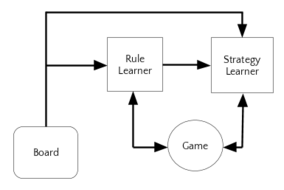
\includegraphics[width=\linewidth]{sys_arch.png}
  \caption{The system architecture with the computational flow.}
  \label{fig:sys_arch}
\end{figure}

\subsection{Rule Learner}
The Rule Learner’s task is to return the valid moves given a certain board state. The board is represented by a $H\times W\times 3$ tensor, where $H$ and $W$ are the board height and width while the third dimension is used to represent the state of each grid cell. This tensor encodes the state of each of the $H \times W$ board cells, which can be:
\begin{itemize}
 \item Empty
 \item Occupied by player 1
 \item Occupied by player 2
\end{itemize}
These states are encoded by the vectors [1 0 0], [0 1 0] and [0 0 1] respectively.

The output is represented by a $H \times W$ matrix. Valid moves are indicated by the respective elements in the matrix having been set to 1. Non-valid moves are represented by 0s.
The RL network maps the input tensor to the output matrix. The network has an input layer with $H \times W \times 3$ units, a single 50-unit fully-connected hidden layer with a $tanh$ activation function, and a fully connected $tanh$ output layer with $H \times W$ units. More information about the train and test process is given in section 3.

\subsection{Strategy Learner}
Similar to DeepMind we used a convolutional neural network to train the Strategy Learner. The network is trained to learn the $Q^(s, a)$, the expected total reward obtained by executing the action $a$ in state $s$ and always picking the optimal actions in future states.

The first layer in this network is the which takes in the state of the board and the valid moves from the rule learner. The board state and valid moves matrix, each of dimension $H \times W$, are stacked to created a single input $2 \times H \times W$

This input is then fed into a convolution layer with 16 filters of size $4 \times 4$. The filters are shifted across the input horizontally and vertically using a stride (shifting offset) of 1. In theory, using a size of $4 \times 4$ should allow a single filters to be able to detect both four-in-a-rows, i.e., a win or loss condition, and three-in-a-rows where one of the players could be about to win.

After the convolution a rectified linear activation function ($\text{max}(0, x)$) is applied. The outputs are then fed into a fully connected layer with 64 nodes and again rectified linear activation. Finally, the outputs of this layer are given to the fully connected output layer with 7 nodes, 1 for each column to play in. A graphical representation of the network can be seen in Figure \ref{fig:strat_learn}.

\begin{figure*}
  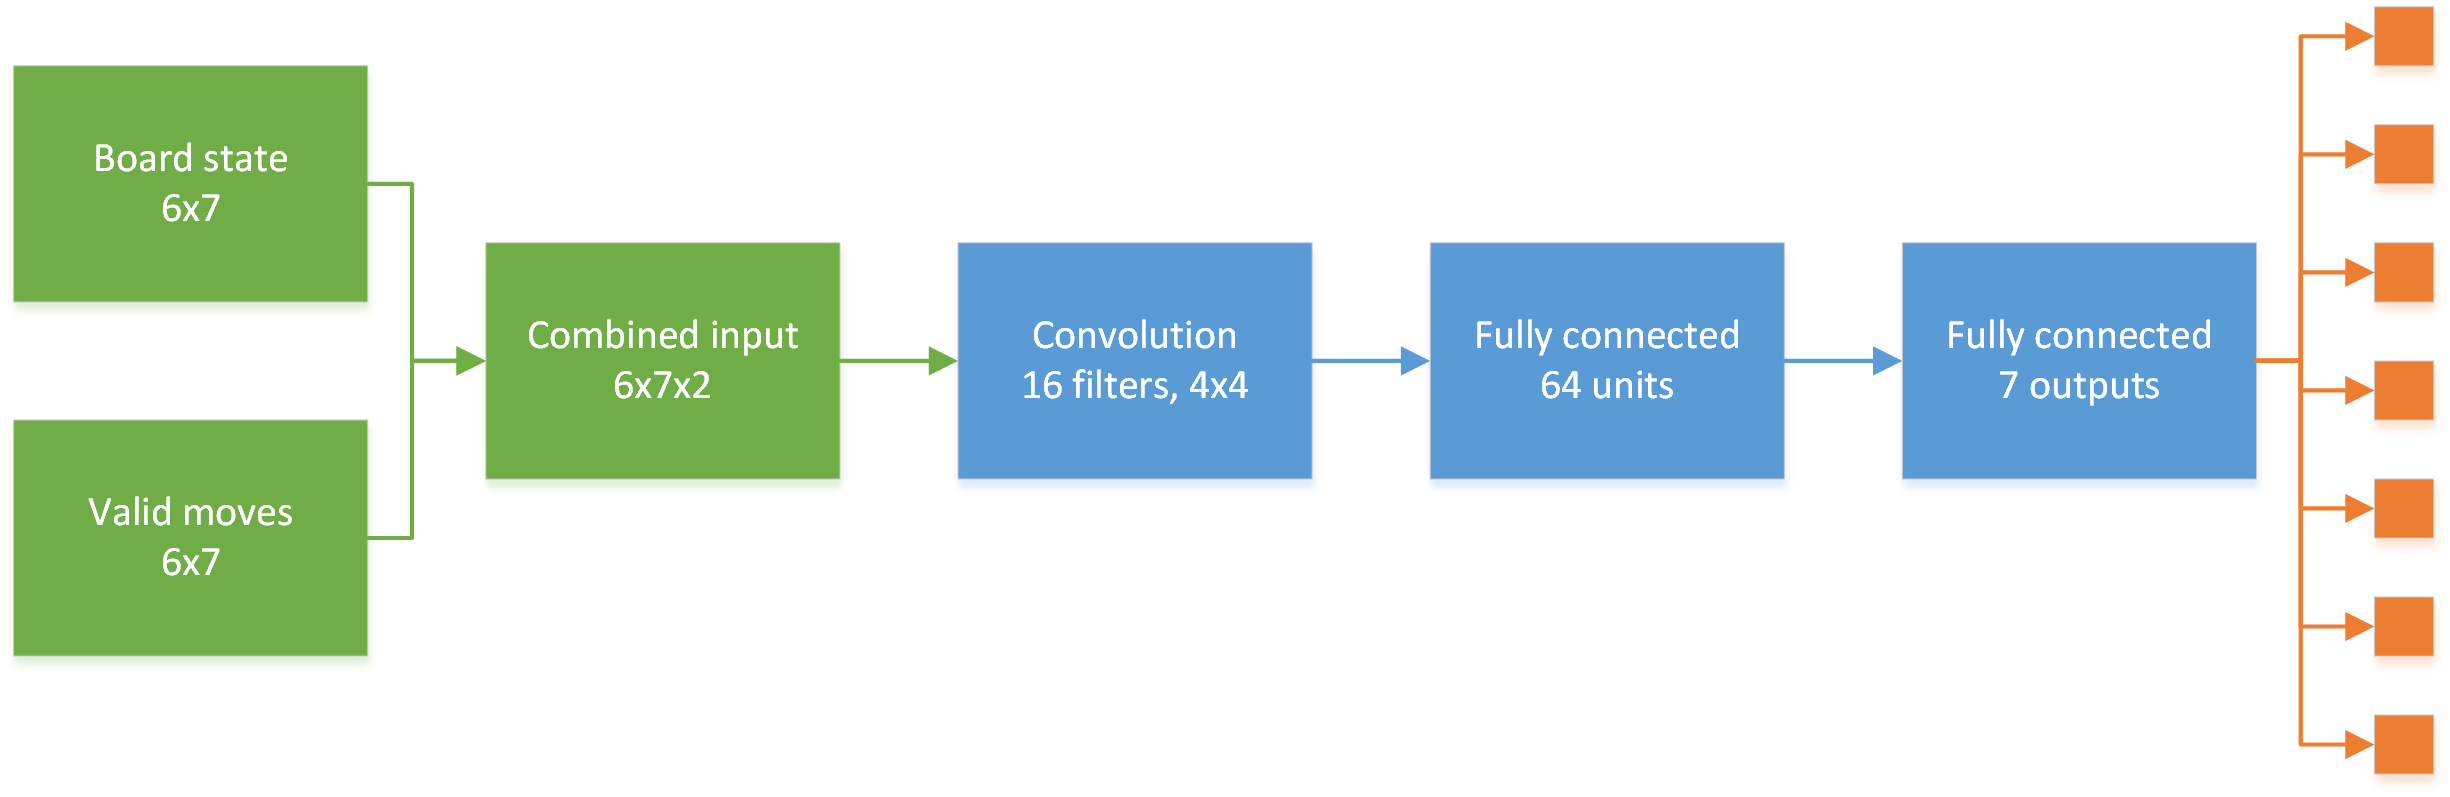
\includegraphics[width=\textwidth]{Network1.png}
  \caption{Strategy Learner network structure}
  \label{fig:strat_learn}
\end{figure*}

\subsection{Training}
The network is trained by having it play games against another player. This player can use the very same network that is currently being trained allowing the network to (indirectly) learn form its own actions, although this is not required.

On every iteration (game step) the network pick an action to execute. With a probability of $\epsilon$ the network selects a random action, with probability $1 - \epsilon$ the action with the highest $Q$-value. $\epsilon$ starts out at 1 and is decreased over time. Initially, selecting random actions is important for the learner to be able to explore the state space. Later on, the learner should fewer random actions to make sure it can reach and explore more advanced game states (instead of losing early on due to randomly selecting bad actions).

When the network loses the game it incurs a reward of -1. If the learner at any time makes an invalid move it directly loses the game and also receives a reward of -1 and. When it wins a game it receives a reward of +1. During most iterations though its action will not directly lead to a win or loss, in which case it receives no reward (0). Finally, in the case of a tie (all columns are full and no player has won) the network receives a final reward of 0.

No discounting of future reward is applied, as the only reward the network will ever receive is at the very end a game. The length of the game is not important.
\section{Experimental Results and Conclusions}

\subsection{Rule Learner}
We used 2000 randomly initialized board states each for our training, validation and testing datasets. All of these were valid board states and there were no repetitions.

We were able to achieve 100\% accuracy (0 Error) on the test set, where the error is the Euclidean distance between the predicted valid moves and actual valid moves (represented as cells containing either a 0 or a 1) averaged over all test set samples.

\subsection{Strategy Learner}
We trained this network over 150 epochs with 25000 episodes per epoch. This resulted in about 90000 games to train on. We were able to see the strategy network understand the valid moves input from the rule learner. To test the network we played against a random AI and a minimax algorithm with varying depths. The results can be seen in Table \ref{table}. 

\begin{table}[h!]
  \begin{center}
    \begin{tabular}{c||c}
    	opponent & result\\
    	\hline
    	\hline
      	random & 95$\%$\\
      	\hline
      	minimax 1 & win\\
      	\hline 
      	minimax 3 & win\\
      	\hline 
      	minimax 5 & lose\\
    \end{tabular}
  \end{center}
  \caption{Performance of the Strategy Learner against different opponents.}
  \label{table}
\end{table}

For the random result we would expect that there are situations that would arise that the network was not trained for and would lose. For the other results, against the minimax algorithm, only one game was played because both our network and the minimax algorithm are deterministic. 

A minimax at a depth of 10 is considered optimal, as it balances searching the tree and speed of the algorithm, however we found that the network was not able to learn a strategy that could beat the minimax at a depth of 5 let alone 10.

The strategy that the network learned does not always pick the optimal move. For example, in the situations below, it should have picked the winning move, but the network does not seem to learn how to win in all situations. This is demonstrated in Figures \ref{state_move_0} and  \ref{state_move_2}.

\begin{figure}
    \makebox[\linewidth]{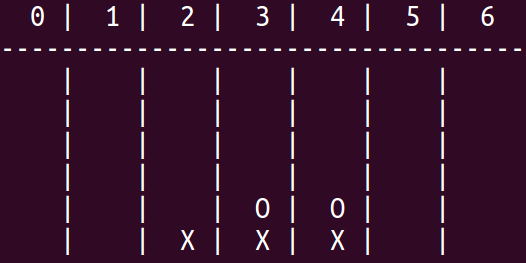
\includegraphics[width=0.5\textwidth]{state1.png}}
    \caption{A state in a game between minimax 3 and our trained network}
    \label{state_move_0}
\end{figure}


\begin{figure}
    \makebox[\linewidth]{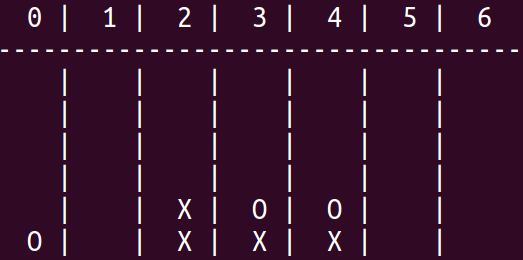
\includegraphics[width=0.5\textwidth]{state2.png}}
    \caption{A second state 2 moves later in a game between minimax 3 and our trained network}
    \label{state_move_2}
\end{figure}


Looking at these states we can see that the network could have won, however it did not pick the best result, confirming that currently the network is not optimal. However, we were able to improve upon random suggest future improvements could yield better results. 
\section{Future Work}
In the future we would like to attempt 3 things, the first being to train on even more games. There are approximately 4.5 trillion board states and we trained over at most 3.78 million. We think that the filters may not have been fully trained resulting in worse performance. 

Another step we would like to try is to adjust the network structure. Currently we are passing the valid moves to the convolution layer. We think that merging the valid moves with the output of the dense layer $lout$ allow it to pick better moves faster. This change would make the network structure look like Figure \ref{fig:struct_future}.

\begin{figure}
  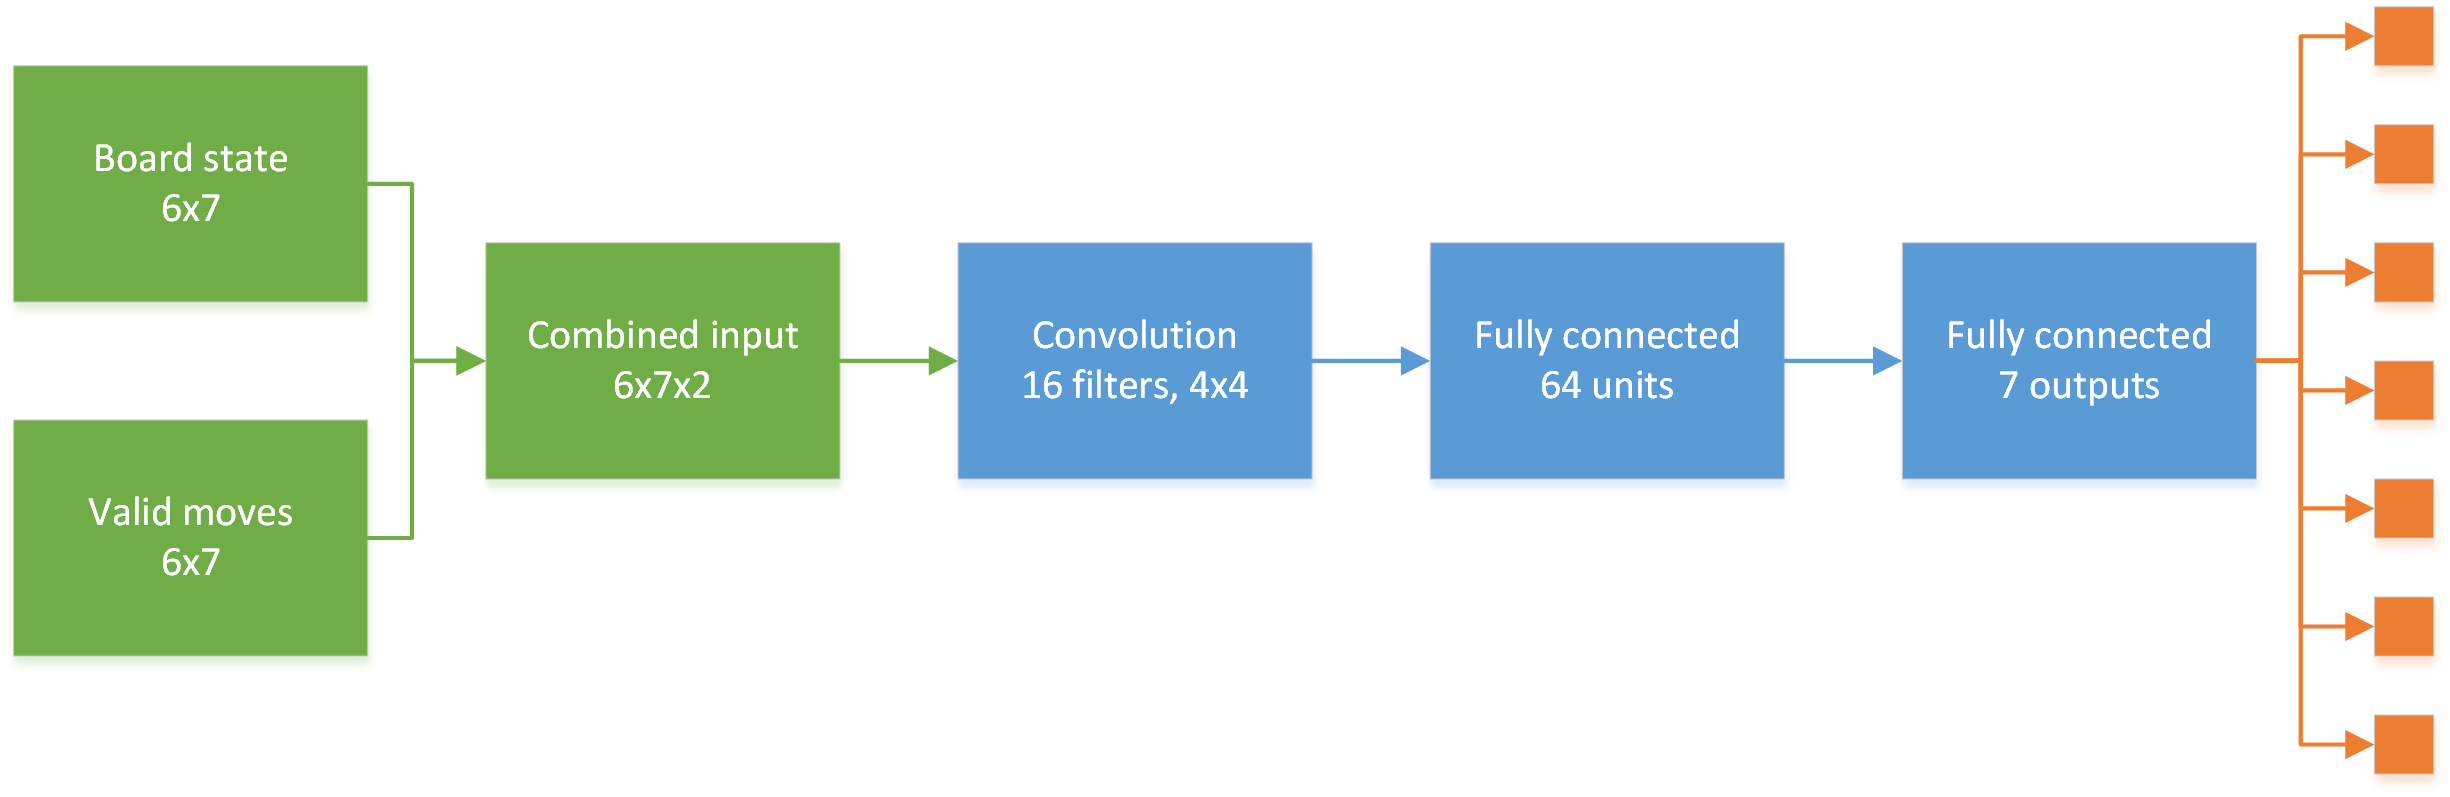
\includegraphics[width=\linewidth]{Network1.png}
  \caption{Possible future network structure}
  \label{fig:struct_future}
\end{figure}

This is just another structure that we could try. Additional structures with more layers could be used to create a better network. 

Finally, we would like to attempt to incorporate memory. Just like a person will try to manipulate the game to get to a state where they know they can win, we want to add that ability to the network. By giving a board state to the network which is close to our current board state and a state from which we have won before we could train the network to use the memory of past games to improve future games performance just like a person would do.

\section{REFERENCES}
[1] Mnih, Volodymyr et al. Playing Atari With Deep Reinforcement Learning. 2014.

[2] Mnih, Volodymyr et al. 'Human-Level Control Through Deep Reinforcement Learning'. Nature 518.7540 (2015): 529-533.

[3] Whitebread, David. 'The Importance Of Play'. N.p., 2012.
  


	\bibliographystyle{ieee}
				  %\bibliographystyle{iclr2016_conference}

%\bibliography{iclr2016_bib}
	
	\bibliography{egbib}


\end{document}
